% isolation-levels.tex

\documentclass{standalone}
\usepackage{tikz}

\usetikzlibrary{shapes, positioning, arrows.meta, decorations.pathmorphing}

\begin{document}
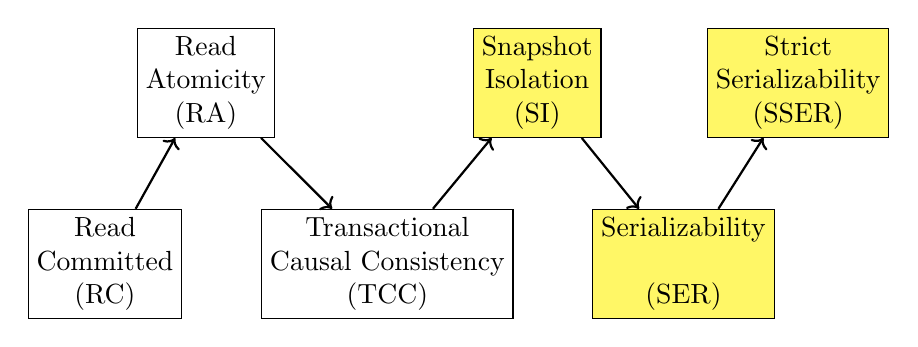
\begin{tikzpicture}[
  node distance = 1.00cm,
	tcm/.style = {draw, rectangle,
	  inner sep = 3pt,
    minimum width = 30pt,
    align = center
    },
	]

  % \node[tcm] (rc) {Read Committed\\\phantom{RC}\\(RC)};
  % \node[tcm, right = of rc] (tcc) {Transactional\\Causal Consistency\\(TCC)};
  % \node[tcm, right = of tcc, fill = yellow!60] (ser) {Serializability\\\phantom{SER}\\(SER)};

  % \node[tcm, above right = 1.60cm and 0.30cm of rc, anchor = center] (ra) {Read Atomicity\\\phantom{RA}\\(RA)};
  % \node[tcm, above right = 1.60cm and 0.30cm of tcc,
    % anchor = center, fill = yellow!60] (si) {Snapshot Isolation\\\phantom{SI}\\(SI)};
  % \node[tcm, above right = 1.60cm and 0.30cm of ser,
    % anchor = center, fill = yellow!60] (sser) {Strict\\Serializability\\(SSER)};

  \node[tcm] (rc) {Read\\Committed\\(RC)};
  \node[tcm, right = of rc] (tcc) {Transactional\\Causal Consistency\\(TCC)};
  \node[tcm, right = of tcc, fill = yellow!60] (ser) {Serializability\\\phantom{SER}\\(SER)};

  \node[tcm, above right = 1.60cm and 0.30cm of rc, anchor = center] (ra) {Read\\Atomicity\\(RA)};
  \node[tcm, above right = 1.60cm and 0.30cm of tcc,
    anchor = center, fill = yellow!60] (si) {Snapshot\\Isolation\\(SI)};
  \node[tcm, above right = 1.60cm and 0.30cm of ser,
    anchor = center, fill = yellow!60] (sser) {Strict\\Serializability\\(SSER)};

  \path[->, thick]
    (rc) edge (ra)
    (ra) edge (tcc)
    (tcc) edge (si)
    (si) edge (ser)
    (ser) edge (sser);
\end{tikzpicture}
\end{document}